Before we introduce the complete workflow to train a network on NCSM ground-state energy sequences, we first have to decide on the network structure to use.
This includes the structure of the input layer, the structure of the output layer, as well as the structure of the hidden layers.

\subsection{Network structure}
NCSM calculations are usually done with multiple different oscillator frequencies $\hbar \Omega$. Different oscillator frequencies result in different convergence rates of the energy sequences, but the limit stays the same. Thus, we want to incorporate more then one frequency into the extrapolation in order to give the maximum amount of information about the interaction and the nucleus into the network.
For that, we do not only try to extrapolate a single energy sequence, but input multiple sequences for different oscillator frequencies into the network.
We decide on 3 energy sequences with given frequencies to input into the network.

In order to determine the structure of the input layer, we must further choose a fixed length of the energy sequences which are put into the network.
For NCSM calculations for heavier nuclei, there are not many $N_\mathrm{max}$ values available, which means that we have to intentionally keep the sequence length small enough.
We decide on energy sequences of length 4.
In summary, the input layer thus has to consist of $L^{(1)} = 3\times 4 = 12$ input neurons.

Since the output of the neural network should be a single real number indicating the extrapolated ground-state energy, the output layer consists of $L^{(N)} = 1$ neuron.

For the hidden layers, there is no generally accepted method of defining the most efficient structure. For the most part, the count of the hidden layers, as well as the count of the neurons in those layers have to be chosen empirically, such that the network neither underfits nor overfits the data. For our framework, we choose $N = 4$ total layers, such that there are two hidden layers of $L^{(2)} = 24$ and $L^{(3)} = 12$ neurons.

% Activation Function
Each layer besides the output layer will be given a \textit{rectifier} activation function (\textit{ReLU}) given by
\begin{equation}
  \sigma(z) = \max(0, z),
\end{equation}
which restricts the activations of the neurons to be positive. This function is chosen because it empirically yields the best results for the extrapolation. Furthermore, it simplifies the calculations on the neural network and with it the computation time. Notice that the activations of the last layer will not get rectified, as the extrapolations, and therefore the network output, should not be limited to positive ground-state energies. As a consequence, the connections of the second-last layer to the last layer will also be responsible for the sign of the extrapolated energy. In \autoref{fig:dataflow}, the data flow of our extrapolation framework is shown.


\begin{figure}[H]
  \centering
  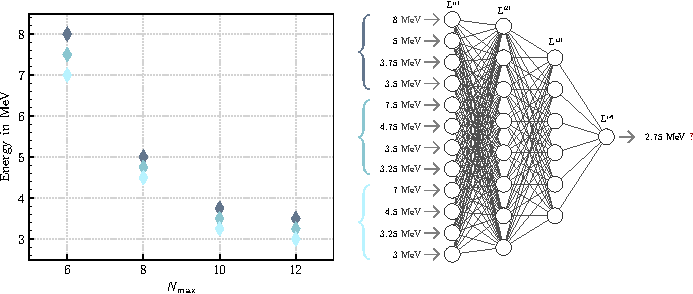
\includegraphics[width=\textwidth]{media/netviz.pdf}
  \caption{Our extrapolation framework visualized. On the left, an examplary formatted input is shown, consisting of three sequences of four nmax values. The data is input into the network, which then outputs an estimation on the common sequence limit. Note that not all neuron in layers $L^{(2)}$ and $L^{(3)}$ are shown for the sake of visibility. In our framework, $L^{(2)} = 24$ and $L^{(3)} = 12$.}
  \label{fig:dataflow}
\end{figure}
% Loss function
\subsection{Other parameters}
The loss function of our network is a standard \textit{Mean Squared Error} (MSE) loss given for a single network input $x$ by
\begin{equation}
  C_x = \norm{f(x)-o}^2,
\end{equation}
where $f(x)$ is the vector of activations of the neurons in the output layer given the input of $x$, and $o$ is the vector of desired activations. The unit of the loss function is therefore $\si[]{\mega\electronvolt\squared}$. For $n$ input samples $x_i$ with desired outputs $o_i$, the loss is averaged over all samples yielding
\begin{equation}
  C = \frac{1}{n}\sum_{i=1}^n C_{x_i}=\frac{1}{n} \sum_{i=1}^{n}\norm{f(x_i)-o_i}^2.
\end{equation}

% Optimization algorithm
For the optimization process, we opt for the \textit{AdamW} algorithm. This is a variant of the \textit{Adam} algorithm \cite{adamw, adam}, which is based on the simple stochastic gradient descent algorithm introduced in \autoref{sec:sgd}. As such, the general optimization process is the same as with stochastic gradient descent.

For gradient-based optimization algorithms, we have to choose a learning rate $\eta$, which determines the ratio of the step size to the value of the gradient. Values of $\eta$ that are too large result in an instability of the optimization algorithm, while values, which are too small, result in smaller step sizes. The learning rate is empirically chosen to be $\eta = 0.01$, such that both extreme cases will be avoided.

Overall, we iterate 20 times (\textit{epochs}) over the training data set, using batch sizes of 512. Since the learning rate can independently be adjusted for each epoch, it is common practice to reduce the learning rate once the optimization has stagnated, such that further optimization may be achieved. In out network training, we decrease the learning rate by a factor of 2, if the loss function as measured by a small set of input data called the \textit{development set} does not decrease by 10\% over 2 epochs (This mechanism is called \textit{learning rate scheduling}).

After the optimization is done, the network is validated using a \textit{validation set}. Here, the loss is computed using all samples in the validation set and compared to a threshold of \SI{0.3}{\mega\electronvolt\squared}. If the loss is smaller than the threshold, the network is suited for our extrapolation. Otherwise, the network will be discarded.

% Implementation
To implement the neural network, we use \textit{pytorch}, which is a machine learning library for Python.

\subsection{Preparation of input data for the training process}
\label{sec:inflate}
The networks have to be trained using energy sequences with known limits. Since it is impossible to calculate the limit using the full Hilbert space, we have to base the training on NCSM sequences which can be calculated to a sufficiently large value of $N_\mathrm{max}$, such that the lowest value for the highest $N_\mathrm{max}$ gives a good enough approximate for the limit. For that, we need to assume that the sequences have more or less converged to the limit. For the training, we thus use NCSM calculations from the nuclei \n{2}{H}, \n{3}{H} and \n{4}{He}. The interactions used are chiral two-body and three-body interactions.

% Generation of input data / Explain inflate
From the NCSM energy sequences, we first generate a large pool of input data which is formatted such that it can be input into the networks. This is necessary since NCSM energy sequences are generally calculated from more than three oscillator frequencies and more values of $N_\mathrm{max}$.

To generate formatted input sequences, we first purge a few exotic cases from the raw input data. Since oscillator frequencies which are too high or too low result in slow converging sequences, we restrict the data of the training process to oscillator frequencies between $\hbar\Omega=\SI{12}{\mega\electronvolt}$ and $\hbar\Omega=\SI{32}{\mega\electronvolt}$. Furthermore, we discard every NCSM calculation done for $N_\mathrm{max} = 0$, since they can result in unphysical energy values. For each nucleus and interaction, we also discard sequences for which the difference between the energy value for the highest $N_\mathrm{max}$ and the limit is higher than \SI{0.05}{\mega\electronvolt} to rule out further special sequences that do not converge enough to the desired limit.
In \autoref{fig:trainingseq}, an example \textit{raw} NCSM calculation for \n{2}{H} is shown, using an SRG evolved Hamiltonian based on a chiral $N^{3}LO$ interaction with two-body interactions and a cutoff at \SI{400}{\mega\electronvolt} by Entem, Machleidt and Nosyk \cite{entemmachleidt}. The flow parameter is given by $\SI{0.04}{\femto\metre^4}$. This is an example of a calculation, which is suitable for training, since the calculations were done for sufficiently large $N_\mathrm{max}$ and the limit could be extracted. We can see the convergence for higher $N_\mathrm{max}$ to a value independent on the oscillator frequency.

\begin{figure}[H]
  \centering
  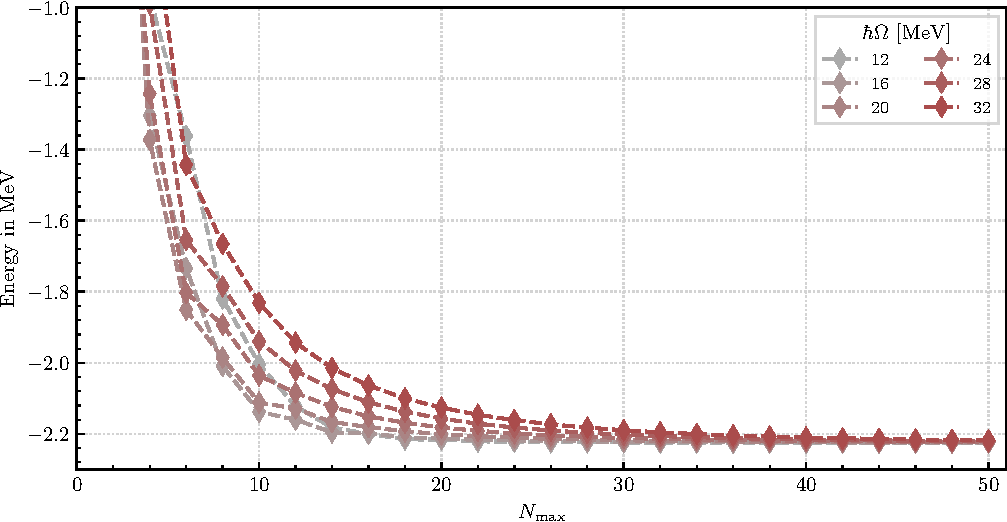
\includegraphics{media/example_sequence.pdf}
  \caption{NCSM results for the $\n{2}{H}$ nucleus. Here, the interaction used for the Hamiltonian is a chiral $N^{3}LO$ interaction with two-body interactions and a cutoff at \SI{400}{\mega\electronvolt} by Entem, Machleidt and Nosyk \cite{entemmachleidt}. Furthermore, the Hamiltionian is SRG evolved using a flow parameter of $\SI{0.04}{\femto\metre^4}$. Each point is the result of a NCSM calculation with a given $N_\mathrm{max}$ and oscillator frequency $\hbar \Omega$.}
  \label{fig:trainingseq}
\end{figure}

Afterwards, we consider every permutation of three frequencies belonging to the six calculated frequencies. Here, we deliberately want the order of the frequencies to not matter, since the network should be trained independent of the order of the inputted data. For each permutation of frequencies, we can choose any four consecutive $N_\mathrm{max}$ values to generate a formatted input sequence.

For any NCSM calculation with $k \geq 3$ Frequencies and $n \geq 4 $ values of $N_\mathrm{max}$, we can thus get $\frac{k!}{(k-3)!} (n-3)$ formatted input sequences into the pool. In the example from above, there are $k=6$ frequencies and $n = 25$, yielding 2640 different formatted sequences. We call this preformatting the \textit{inflation} process of the input data. With each inflated sequence coming from the same NCSM calculation, we associate the same limit extracted as the minimum value of the maximum $N_\mathrm{max}$, which will be used as the target output of the network in the training process.

% Creation of Train / Validate / Dev Set
This large pool of inflated sequences is the basis for the complete training of a network, i.e. for the training itself, but also for the validation and the development set. As the training set should be very large to encorporate as many different sequences into the network as possible, we draw 200,000 random samples from the pool. For the validation of the network, we draw 10,000 random samples and for the development set, we draw 5,000 samples.

Even though the training set will be of a large size, all the samples are derived from a small list of nuclei, for which NCSM calculations up to a high enough $N_\mathrm{max}$ are possible to extract a meaningful limit. As a consequence, all the inflated sequences only cover a small range of absolute energy values as well as a small range of convergence rates. In order to make the network prediction independent of the absolute energy values and the convergence rates, every sample is also multiplied by a randomly chosen constant, to vary the convergence rate, and shifted by a randomly chosen constant, to vary the absolute energies in the sequence. For our work, the multiplier is chosen uniformly from the interval $[0.5, 2]$, and the shift is chosen uniformly from $[\SI{-10}{\mega\electronvolt}, \SI{10}{\mega\electronvolt}]$.
